\chapter{ゲージ不変性と荷電粒子の運動}

\lectureoverview{磁場は発散がゼロであるため、ベクトルポテンシャルによって表すことができる。その表現は一意的ではないが、まさにそれによって磁気的な力を作用原理に取り入れることが可能になる。我々はローレンツ力を導出し、正準運動量と力学的運動量を区別し、ハミルトニアンを構成し、2つの異なるゲージを用いて一様磁場中の運動を解く。講義の最後には、この粒子力学がマクスウェル理論、磁気単極子、位相空間の力学というより大きな主題の中にどのように位置づけられるかを示す。}

\section{力学の講義における最後の一歩}

講義は小さな日程上の驚きから始まる。予定では、磁場中の荷電粒子を終わらせ、おそらく電場を加え、その後、次の会合に何を残すかを決めることになっている。聴衆は、これがすでに第10回の講義であると指摘する。その場合、課題はより明確になる。磁場の問題を終わらせ、それによって古典力学の形式的構造を締めくくるのである。

まず簡単な復習から始める。磁場はベクトル場であり、
\begin{equation}
  \mathbf B=\mathbf B(\mathbf x),
  \qquad
  B_i(\mathbf x)=(B_x,B_y,B_z),
\end{equation}
各点で大きさと向きをもつ。この講義では、外部の電場と磁場は静的であると仮定する。この制限は明確さのために置かれるのであって、電磁場が常に時間に依存しないというわけではない。

また、制約がある。
\begin{equation}
  \nabla\cdot\mathbf B=0.
\end{equation}
流体の類推では、これは磁束が外へ注ぎ出す管の端も、それが消えていく排水口も存在しないことを意味する。通常の古典電磁気学では、磁気的な源も吸い込みも存在しない。実験は素磁気単極子を確立していないが、講義では、より完全な理論がそれを含む可能性を繰り返し開いたままにしている。

\begin{figure}[htbp]
\centering
\includegraphics[width=0.78\textwidth]{lecture_10_figure_02.png}
\caption{場の成分、源のない条件\(\nabla\cdot\mathbf B=0\)、およびベクトルポテンシャルによる表現が、講義の冒頭に一緒に現れる。}
\lectureframe{00:04:56}
\end{figure}

場を提案するたびに発散を確認する代わりに、制約を自動的に満たすことができる。次のように書く。
\begin{equation}
  \boxed{\mathbf B=\nabla\times\mathbf A}.
\end{equation}
すると、恒等式
\begin{equation}
  \nabla\cdot(\nabla\times\mathbf A)=0
\end{equation}
がその記帳を我々の代わりに行う。新しい場\(\mathbf A\)がベクトルポテンシャルである。

\section{自動的な制約の代償}

\(\mathbf A\)を導入すると、1つの問題が解決され、別の問題が生じる。すなわち、それは一意的ではない。任意のスカラー関数\(S(\mathbf x)\)に対して、
\begin{equation}
  \mathbf A'=\mathbf A+\nabla S
\end{equation}
は同じ回転をもつ。なぜなら、
\begin{equation}
  \nabla\times(\nabla S)=0.
\end{equation}
だからである。したがって、\(\mathbf A\)と\(\mathbf A'\)は同じ磁場を記述する。十分に単純な領域では、これが完全な局所的な曖昧さである。すなわち、2つのベクトルポテンシャルが同じ回転をもつならば、それらの差は局所的に勾配である。大域的な位相幾何学は複数のパッチを必要としたり、さらなる微妙さを許したりしうるが、ここで考える場にはそれらのいずれも必要ない。

特定の代表は\emph{ゲージ}と呼ばれ、代表を変えることは\emph{ゲージ変換}である。場\(\mathbf B\)は変化しないので、ゲージ不変である。作業原理は、観測可能な物理がどの代表を選んだかに依存してはならないというものである。我々は\(\mathbf A\)を導入して記述を拡大し、その後、ゲージ不変な予測を要求することによって記述上の冗長性を取り除いた。

\subsection{一様場に対する3つのゲージ}

講義は直ちにこの考えを具体化する。一様な磁場が\(z\)軸に沿って向くように座標を選ぶ。
\begin{equation}
  \mathbf B=B\hat{\mathbf z},
  \qquad
  B_x=B_y=0,
  \qquad
  B_z=B,
\end{equation}
ここで\(B\)は定数である。最初のベクトルポテンシャルは
\begin{equation}
  \mathbf A^{(1)}=(0,Bx,0).
\end{equation}
である。実際、
\begin{equation}
  (\nabla\times\mathbf A^{(1)})_z
  =
  \frac{\partial A_y^{(1)}}{\partial x}
  -
  \frac{\partial A_x^{(1)}}{\partial y}
  =B.
\end{equation}
第2の選択は
\begin{equation}
  \mathbf A^{(2)}=(-By,0,0),
\end{equation}
であり、これに対して
\begin{equation}
  (\nabla\times\mathbf A^{(2)})_z
  =
  0-\frac{\partial(-By)}{\partial y}
  =B.
\end{equation}

両者の間を移るには、
\begin{equation}
  S=Cxy,
  \qquad
  \nabla S=(Cy,Cx,0).
\end{equation}
を取る。\(\mathbf A^{(1)}\)から出発すると、変換された成分は
\begin{equation}
  A_x'=Cy,
  \qquad
  A_y'=(B+C)x,
  \qquad
  A_z'=0.
\end{equation}
である。\(C=-B\)という選択は\(\mathbf A^{(2)}\)を与える。\(C=-B/2\)という選択は対称ゲージ
\begin{equation}
  \mathbf A^{(\mathrm{sym})}
  =
  \left(-\frac{B}{2}y,\frac{B}{2}x,0\right)
  =
  \frac12\,\mathbf B\times\mathbf r.
\end{equation}
を与える。3つとも同じ回転をもつ。後で我々は意図的に最初の2つに戻る。なぜなら、それぞれが異なる並進対称性を明らかにするからである。

\begin{classroomqa}
\audiencequestion{ベクトルポテンシャルは一様磁場と同じ対称性をもてるか。}
\lecturerresponse{磁場と同じように空間的に一定であることはできない。なぜなら、一定のベクトルポテンシャルは回転がゼロだからである。また、単一のゲージは、非零の一様場のすべての並進対称性を同時に明示することもできない。対称ゲージは\(z\)軸のまわりの回転を明示するので、正確な教訓は、すべての対称性が\(\mathbf A\)に欠けていなければならないということではなく、ポテンシャルが物理場のすべての対称性を一度に示す必要はないということである。}
\end{classroomqa}

族 \(S=Cxy\) は単なる一例にすぎない。より一般には、適切な領域で \(\mathbf A\) の一成分を消すなど、有用なゲージ条件を課すことができる。\emph{ゲージ} という名称は、この自由度を単位の局所的な変更と解釈しようとした不成功な試みに歴史的に由来する。その解釈は放棄されたが、名称は残った。

\begin{classroomqa}
\audiencequestion{ゲージ変換とは常にスカラーの勾配を加えることを意味するのか。}
\lecturerresponse{ここで用いたのは静的な電磁ベクトルポテンシャルに対する変換である。他のゲージ理論にはより複雑な変換があり、重力においては座標の変更がしばしばゲージ変更として記述される。それは物理的な幾何が座標のラベルに依存しえないからである。しかし本章では、ゲージ変換とは \(\mathbf A\mapsto\mathbf A+\nabla S\) を意味する。}
\end{classroomqa}

\begin{classroomqa}
\audiencequestion{あるゲージが別のゲージより計算上優れていることはありうるか。}
\lecturerresponse{しばしばある。対称性や保存則があるゲージでは明白であり、別のゲージでは隠れていることがある。それは単なる抽象的な可能性ではない。この講義の後半で、あるゲージでは \(y\) が循環的になり、別のゲージでは \(x\) が循環的になる。どちらの計算も同じ軌道を記述している。}
\end{classroomqa}

\begin{classroomqa}
\audiencequestion{この曖昧さは固有空間の選択や固有値の決定と関係があるのか。}
\lecturerresponse{ここでは直接の関係は必要ない。どちらの主題も有用な数学的選択を伴うが、固有基底の変更と電磁ゲージ変換は異なる構造である。}
\end{classroomqa}

\section{磁場のラグランジアン}

ここで力学に戻る。議論する対象は、与えられた磁場中を運動する点粒子のラグランジアンであり、まだ電磁場そのもののラグランジアンではない。講義で用いた単位の慣習では、
\begin{equation}
  L
  =
  \frac{m}{2}
  \left(\dot x^2+\dot y^2+\dot z^2\right)
  +
  \frac{e}{c}
  \left(
    A_x\dot x+A_y\dot y+A_z\dot z
  \right).
\end{equation}
ベクトル記法では、
\begin{equation}
  \boxed{
  L=\frac12 m\mathbf v^2+\frac{e}{c}\mathbf A(\mathbf x)\cdot\mathbf v
  }.
\end{equation}
係数 \(e\) は粒子の電荷である。明示的な \(c\) は単位の慣習に依存する。構造的な内容は速度に依存する結合 \(\mathbf A\cdot\mathbf v\) である。

\begin{figure}[htbp]
\centering
\includegraphics[width=0.86\textwidth]{lecture_10_figure_03.png}
\caption{磁場中の粒子のラグランジアンは、3つの速度結合を見える形に保ちながら成分ごとに書かれている。}
\lectureframe{00:25:29}
\end{figure}

最初はこの項は導出されるのではなく提案される。これを試してどのような方程式が得られるかを見るよう促されている。\(\mathbf B\) から直接作られた項も試すことはできるが、それは \(\mathbf B\) の導関数を生み、ローレンツ力にはならない。ベクトルポテンシャルは経路に正しく結合する局所的な対象である。

\subsection{ゲージシフトが軌道を変えない理由}

作用を変分する前に、ゲージ変換が作用に何をするかを確認しよう。初期と最終の時空点を固定すると、
\begin{equation}
  \mathcal S[\mathbf x]
  =
  \int_{t_i}^{t_f}L\,dt.
\end{equation}
\(\mathbf A\mapsto\mathbf A+\nabla S\) の下で、変化は
\begin{align}
  \Delta\mathcal S
  &=
  \frac{e}{c}
  \int_{t_i}^{t_f}
  \nabla S(\mathbf x)\cdot\dot{\mathbf x}\,dt\\
  &=
  \frac{e}{c}
  \int_{t_i}^{t_f}\frac{dS(\mathbf x(t))}{dt}\,dt\\
  &=
  \frac{e}{c}
  \left[
    S(\mathbf x_f)-S(\mathbf x_i)
  \right].
\end{align}
したがって作用の数値は変化する。しかし加えられた項は固定された端点のみに依存し、経路の変分される内部には依存しない。その変分はゼロであり、停留軌道を変えることはできない。

\begin{classroomqa}
\audiencequestion{方程式がゲージ不変であるとはどういう意味か。}
\lecturerresponse{オイラー--ラグランジュの計算の後、\(\mathbf A\) は \(\mathbf B\) の成分として認識される回転の組み合わせにのみ現れなければならない。ポテンシャル自体は変化してもよく、作用は端点項だけずれてもよいが、物理的な軌道と力の法則は変わらないままでなければならない。}
\end{classroomqa}

\section{運動量の二つの概念}

オイラー--ラグランジュ方程式は次のように書ける。
\begin{equation}
  \dot p_i=\frac{\partial L}{\partial x_i},
  \qquad
  p_i=\frac{\partial L}{\partial\dot x_i}.
\end{equation}
ここで二つの運動量を区別しなければならない。よく知られた力学的運動量は
\begin{equation}
  \boldsymbol{\pi}=m\mathbf v.
\end{equation}
正準運動量はラグランジアンによって定義される。
\begin{equation}
  p_i
  =
  m\dot x_i+\frac{e}{c}A_i.
\end{equation}
したがって
\begin{equation}
  \boxed{
  \boldsymbol{\pi}
  =
  \mathbf p-\frac{e}{c}\mathbf A
  =
  m\mathbf v
  }.
\end{equation}
自由粒子、あるいは通常の位置に依存するポテンシャルの場合、正準運動量と力学的運動量は一致する。磁気的相互作用は速度に依存するので、もはや一致しない。

\begin{figure}[htbp]
\centering
\includegraphics[width=0.78\textwidth]{lecture_10_figure_04.png}
\caption{黒板は正準定義 \(p_i=\partial L/\partial\dot x_i\) を \(m\dot x_i\) から分離し、軌道に沿ってそれを微分し始める。}
\lectureframe{00:37:33}
\end{figure}

この区別はそれ自体のための用語ではない。正準運動量はハミルトンの方程式、ポアソン括弧、および循環座標に関連する保存則に入る量である。力学的運動量は直接測定可能な質量と速度の積である。

\begin{classroomqa}
\audiencequestion{\((e/c)\mathbf A\cdot\mathbf v\)は運動エネルギーか、それともポテンシャルエネルギーか。また、それを加えるべきか引くべきかをどうやって見分けるのか。}
\lecturerresponse{それは通常の運動エネルギーでも、通常の位置に依存するポテンシャルでもない。速度に依存する相互作用である。この段階では、その符号は提案された結合の一部であり、その符号を変えることは電荷の符号または\(\mathbf A\)の符号を反転させることに等しい。決定的な検証は、そこから導かれる力の法則である。}
\end{classroomqa}

\section{ローレンツ力に至る代数}

講義では1つの成分をゆっくりと計算する。\(p_x\)について、
\begin{equation}
  p_x=m\dot x+\frac{e}{c}A_x(\mathbf x).
\end{equation}
外部場は静的であっても、\(A_x(\mathbf x(t))\)は粒子が運動するにつれて変化する。その全時間微分は
\begin{equation}
  \frac{dA_x}{dt}
  =
  \frac{\partial A_x}{\partial x}\dot x
  +
  \frac{\partial A_x}{\partial y}\dot y
  +
  \frac{\partial A_x}{\partial z}\dot z.
\end{equation}
したがって、
\begin{equation}
  \dot p_x
  =
  m\ddot x
  +
  \frac{e}{c}
  \left(
    \partial_xA_x\,\dot x
    +
    \partial_yA_x\,\dot y
    +
    \partial_zA_x\,\dot z
  \right).
\end{equation}
オイラー--ラグランジュ方程式の右辺は
\begin{equation}
  \frac{\partial L}{\partial x}
  =
  \frac{e}{c}
  \left(
    \partial_xA_x\,\dot x
    +
    \partial_xA_y\,\dot y
    +
    \partial_xA_z\,\dot z
  \right).
\end{equation}
項\(\partial_xA_x\,\dot x\)は相殺する。残ったものを速度成分ごとにまとめると
\begin{align}
  m\ddot x
  &=
  \frac{e}{c}
  \left[
    \left(\partial_xA_y-\partial_yA_x\right)\dot y
    +
    \left(\partial_xA_z-\partial_zA_x\right)\dot z
  \right].
\end{align}

\begin{figure}[htbp]
\centering
\includegraphics[width=0.80\textwidth]{lecture_10_figure_05.png}
\caption{完成した\(x\)成分の計算。ベクトルポテンシャルの微分が回転の組み合わせにまとまった。}
\lectureframe{00:46:41}
\end{figure}

\begin{align}
  B_y&=\partial_zA_x-\partial_xA_z,\\
  B_z&=\partial_xA_y-\partial_yA_x,
\end{align}
を用いると
\begin{equation}
  m a_x
  =
  \frac{e}{c}
  \left(B_zv_y-B_yv_z\right)
  =
  \frac{e}{c}
  (\mathbf v\times\mathbf B)_x.
\end{equation}
が得られる。\(y\)と\(z\)についても同じ計算を行うと
\begin{equation}
  \boxed{
  m\mathbf a=\frac{e}{c}\,\mathbf v\times\mathbf B
  }.
\end{equation}
これが磁気ローレンツ力の法則である。講義では完全な方程式をニュートン--ローレンツ方程式と呼ぶ。ニュートンが\(m\mathbf a\)を与え、ローレンツが磁気力を与える。

この結果は計算前に提示された3つの検証すべてに合格する。新しい項は非零の力を生み出す。力はゲージ不変である。なぜなら\(\nabla\times\mathbf A=\mathbf B\)だけが生き残るからである。そして、ベクトルポテンシャルは冗長ではあるが、磁気力に作用原理を与えた。相互作用において\(\mathbf A\)を\(\mathbf B\)に置き換えると、\(\mathbf B\)の回転の組み合わせが生じ、この法則を再現しないであろう。

\section{ハミルトニアンとエネルギーの意味}

次の問題は、同じ系がハミルトニアンによる記述を持つかどうかである。
\begin{align}
  p_x&=m\dot x+\frac{e}{c}A_x,\\
  p_y&=m\dot y+\frac{e}{c}A_y,\\
  p_z&=m\dot z+\frac{e}{c}A_z.
\end{align}
から始める。これらの関係は逆に解くことができる。
\begin{align}
  \dot x&=\frac{1}{m}\left(p_x-\frac{e}{c}A_x\right),\\
  \dot y&=\frac{1}{m}\left(p_y-\frac{e}{c}A_y\right),\\
  \dot z&=\frac{1}{m}\left(p_z-\frac{e}{c}A_z\right).
\end{align}
ルジャンドル変換は
\begin{equation}
  H=\sum_i p_i\dot x_i-L.
\end{equation}
である。代入と相殺により
\begin{equation}
  \boxed{
  H(\mathbf x,\mathbf p)
  =
  \frac{1}{2m}
  \left(
    \mathbf p-\frac{e}{c}\mathbf A(\mathbf x)
  \right)^2
  }.
\end{equation}
が得られる。

\begin{figure}[htbp]
\centering
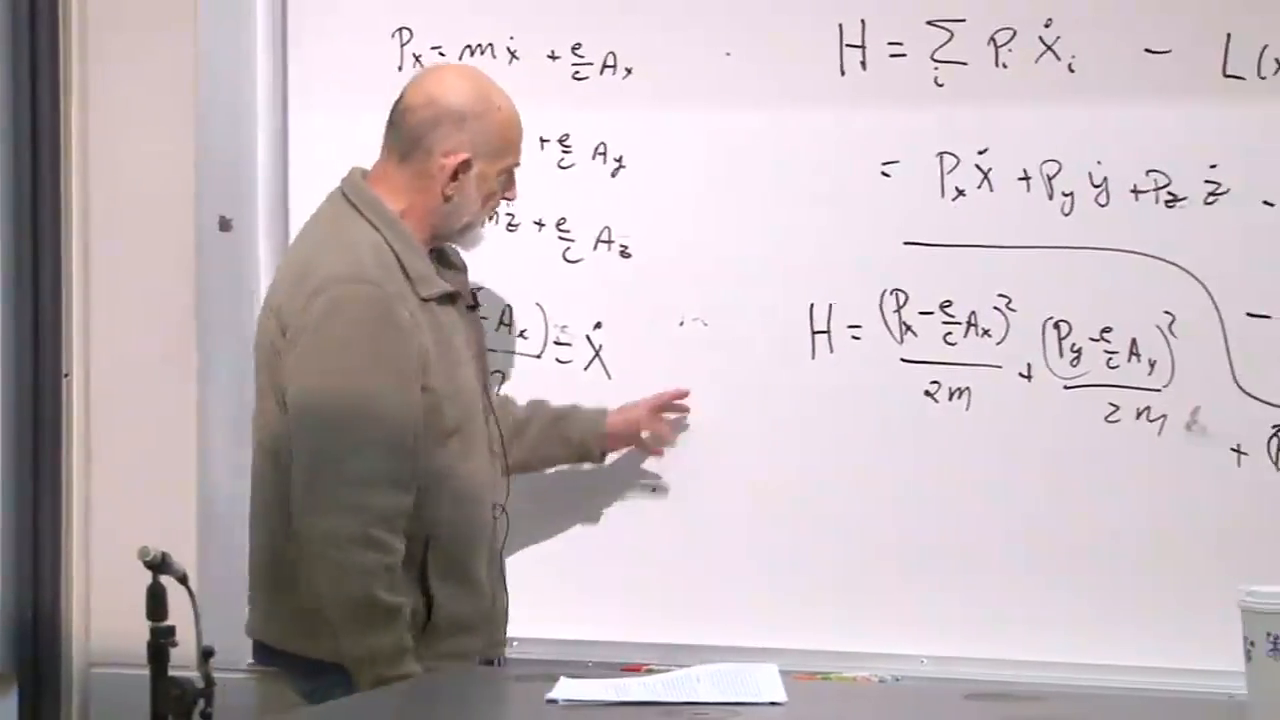
\includegraphics[width=0.86\textwidth]{lecture_10_figure_06.png}
\caption{完成したハミルトニアンの構成では、左辺に3つの正準運動量が保たれ、右辺に最小結合された平方が現れる。}
\lectureframe{00:53:05}
\end{figure}

正準変数で書くと、これは自由粒子のハミルトニアンとは異なる。しかし、物理的な速度で書くと、
\begin{equation}
  H=\frac{\boldsymbol{\pi}^{\,2}}{2m}
  =\frac12m\mathbf v^2.
\end{equation}
矛盾はない。同じ数値のエネルギーが\((\mathbf x,\mathbf p)\)の異なる関数で表されるため、エネルギーが依然として通常の運動エネルギーに等しくても、ハミルトンの方程式は異なる。

場が静的であるから、\(H\)は保存される。したがって速さは一定である。ローレンツ力はこの事実を明白にする。
\begin{equation}
  \frac{d}{dt}\left(\frac12mv^2\right)
  =
  m\mathbf v\cdot\mathbf a
  =
  \frac{e}{c}\,
  \mathbf v\cdot(\mathbf v\times\mathbf B)
  =0.
\end{equation}
磁場は運動の向きを変えるが、速度の大きさは変えない。軌道を曲げるが仕事をしない。

\section{ゲージを変えて解く一様場}

休憩の後、再び一様場
\begin{equation}
  \mathbf B=B\hat{\mathbf z}.
\end{equation}
を考える。目標は単に見慣れた軌道を解くことではない。ゲージを選ぶことで対称性の計算がほとんど労力なしにできる理由を示すことである。

\subsection{第一のゲージ：y座標とz座標が循環的}


\begin{equation}
  A_x=A_z=0,
  \qquad
  A_y=Bx.
\end{equation}
を取る。すると
\begin{equation}
  L
  =
  \frac{m}{2}
  \left(\dot x^2+\dot y^2+\dot z^2\right)
  +
  \frac{eB}{c}x\dot y.
\end{equation}
座標\(y\)と\(z\)は陽に現れない。それらは循環的であるから、その正準運動量は保存される。\(z\)について、
\begin{equation}
  p_z=m\dot z,
  \qquad
  \dot p_z=0,
\end{equation}
したがって
\begin{equation}
  a_z=0.
\end{equation}
粒子は場に沿って一様に運動する。

\(y\)について、
\begin{equation}
  p_y=m\dot y+\frac{eB}{c}x,
  \qquad
  \dot p_y=0.
\end{equation}
したがって
\begin{equation}
  m a_y+\frac{eB}{c}v_x=0,
  \qquad
  \boxed{m a_y=-\frac{eB}{c}v_x}.
\end{equation}

\begin{figure}[htbp]
\centering
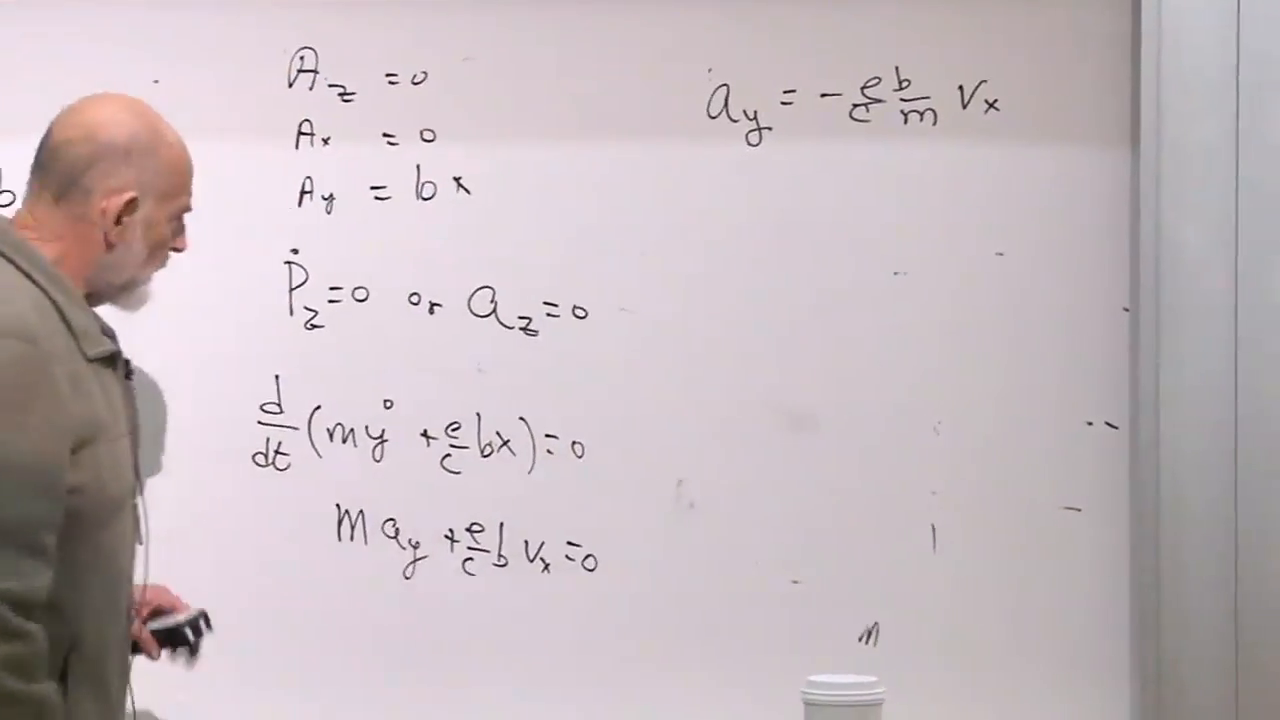
\includegraphics[width=0.84\textwidth]{lecture_10_figure_07.png}
\caption{ゲージ\(A_y=Bx\)において、黒板には保存される\(p_z\)と\(p_y\)、およびその結果得られるローレンツ力の\(y\)成分が記録されている。}
\lectureframe{01:03:50}
\end{figure}

\subsection{第二のゲージ：x座標が循環的}

次に
\begin{equation}
  A_x=-By,
  \qquad
  A_y=A_z=0.
\end{equation}
に切り替える。ラグランジアンは
\begin{equation}
  L
  =
  \frac{m}{2}
  \left(\dot x^2+\dot y^2+\dot z^2\right)
  -
  \frac{eB}{c}y\dot x.
\end{equation}
となる。今度は\(x\)が循環的である。
\begin{equation}
  p_x=m\dot x-\frac{eB}{c}y,
  \qquad
  \dot p_x=0.
\end{equation}
したがって
\begin{equation}
  \boxed{m a_x=\frac{eB}{c}v_y}.
\end{equation}
第一のゲージの結果および\(a_z=0\)と合わせると、これはまさに
\begin{equation}
  m\mathbf a=\frac{e}{c}\mathbf v\times B\hat{\mathbf z}.
\end{equation}
である。

\begin{figure}[htbp]
\centering
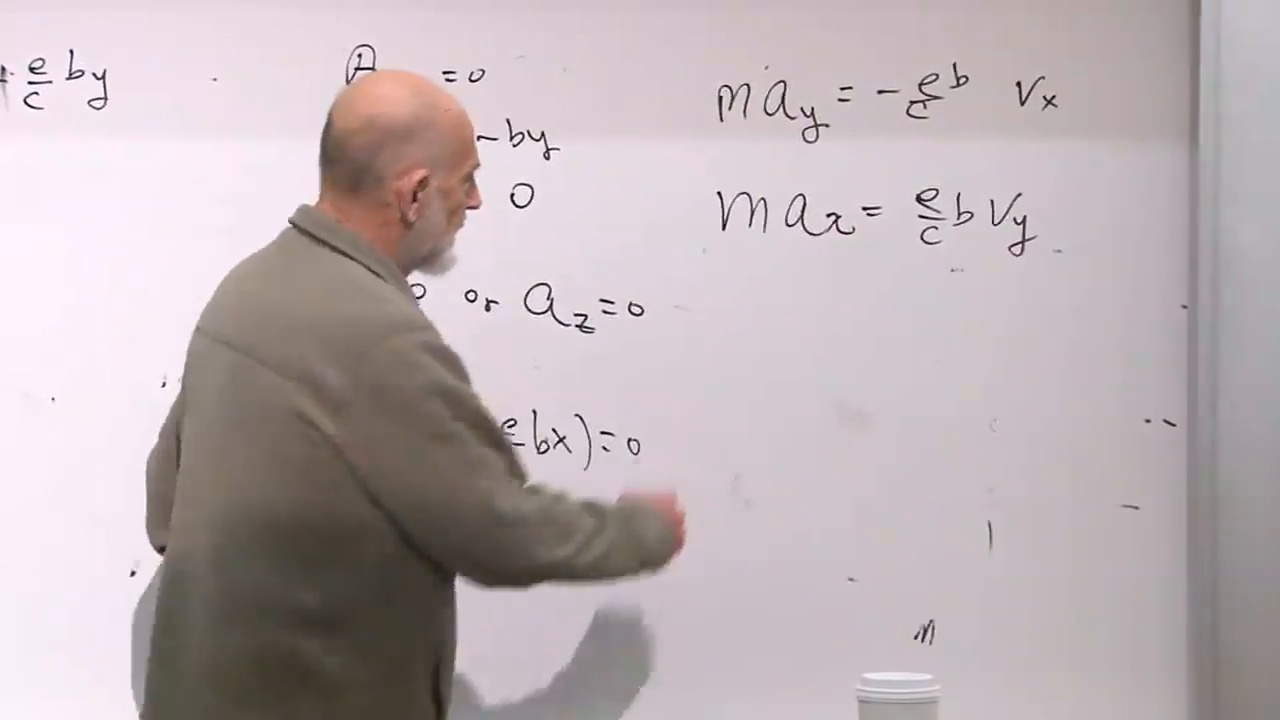
\includegraphics[width=0.84\textwidth]{lecture_10_figure_08.png}
\caption{ゲージを切り替えると、ローレンツ力の横成分が両方とも見える。それぞれが異なるゲージにおける正準運動量の保存則として現れた。}
\lectureframe{01:08:05}
\end{figure}

物理的な並進対称性は終始存在していた。ゲージの選択は、その対称性のどの部分が通常の循環座標として顕在化するかを変えただけである。これが、測定可能な加速度は同じままでありながら、正準運動量があるゲージでは保存され、別のゲージでは異なる形をとり得る理由である。

\begin{classroomqa}
\audiencequestion{正準運動量の成分はゲージ不変か。それらは直接に物理的か。}
\lecturerresponse{否。\(\mathbf A\mapsto\mathbf A+\nabla S\)の下で、正準運動量は\((e/c)\nabla S\)だけ変化する。力学運動量\(m\mathbf v=\mathbf p-(e/c)\mathbf A\)はゲージ不変であり、粒子の速度に直接結びついている。それでも正準運動量は不可欠である。なぜなら、それはハミルトンの方程式とポアソン括弧が用いる変数だからである。}
\end{classroomqa}

\section{一様磁場中の軌道}

形式的な作業は終わった。では運動を見てみよう。まず\(v_z=0\)と仮定すると、粒子は\(xy\)面にとどまる。加速度は速度に垂直であり、その大きさは一定である。
\begin{equation}
  |\mathbf a|
  =
  \frac{|e|}{mc}vB.
\end{equation}
一定の速さで運動し、速度に常に垂直な一定の大きさの加速度をもつ粒子は、円運動をする。

\(r\)を半径とすると、向心加速度は\(v^2/r\)である。大きさを等置すると
\begin{equation}
  m\frac{v^2}{r}
  =
  \frac{|e|}{c}vB,
\end{equation}
したがって
\begin{equation}
  \boxed{
  r=\frac{mcv}{|e|B}
  }.
\end{equation}
講義ではまず\(c\)を欠いた表式を書き、選んだローレンツ力の規約との不一致に気づき、それを復元する。\(eB\)の符号が回転の向きを決める。半径自体は正である。

\begin{figure}[htbp]
\centering
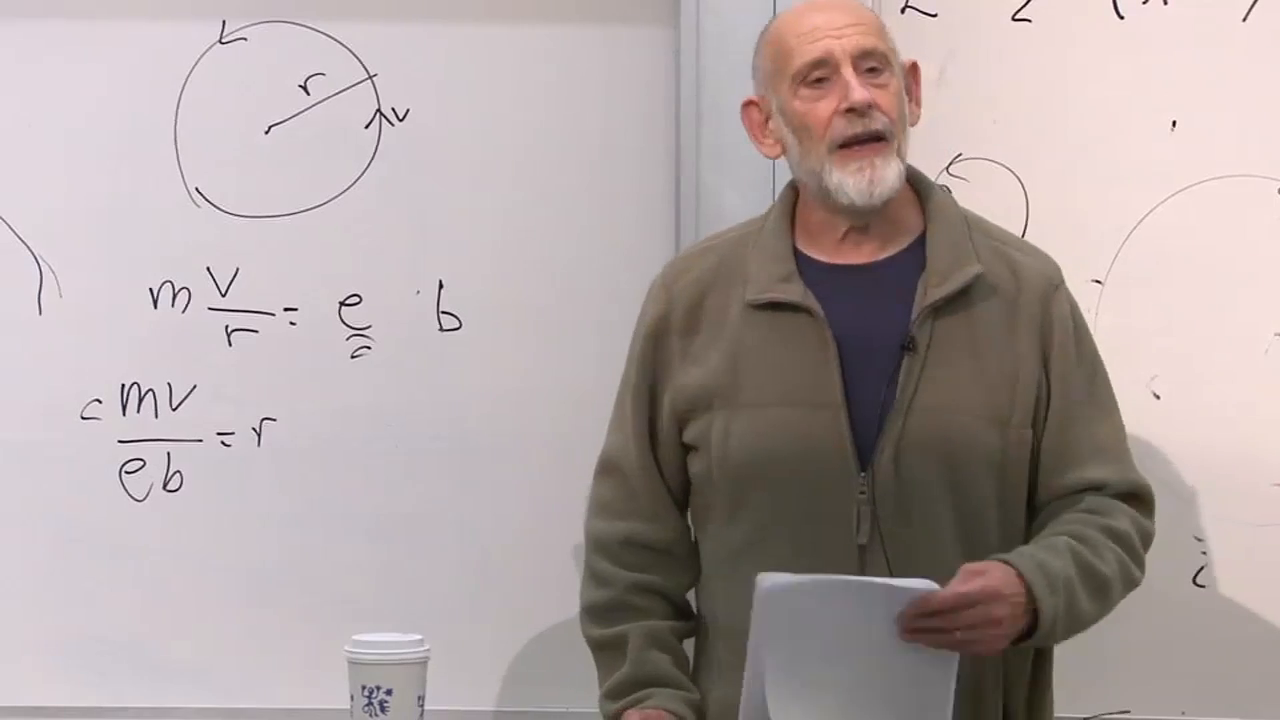
\includegraphics[width=0.84\textwidth]{lecture_10_figure_09.png}
\caption{欠けていた\(c\)の因子が復元された後の、円軌道、接線速度、半径の関係。}
\lectureframe{01:16:50}
\end{figure}

磁場は速さと半径の関係を定めるが、円の中心は定めない。中心は横断面内のどこにでもありうる。横方向の速さが大きいほど軌道は大きくなり、電荷または磁場が大きいほど軌道はより小さくなる。

\(v_z\neq0\)ならば、横方向の運動は円形のままであり、一方\(z\)は一様に進む。これら二つの運動を組み合わせると、磁場の方向のまわりの螺旋が得られる。\editorialnote{講義では二つの要素を別々に導く。すなわち\(a_z=0\)と横方向の円運動である。それらの組み合わせが述べられた螺旋軌道である。}

\section{結合はどこから来たのか。}

軌道の計算は、聴衆に最初に戻るよう促す。項\((e/c)\mathbf A\cdot\mathbf v\)は単に前もって知られていたのか。正直な答えは、論理的に整合するいくつかの出発点が利用可能である、というものである。

\begin{classroomqa}
\audiencequestion{われわれは磁場のラグランジアンを単に知っていて、それを書き下しただけなのか。}
\lecturerresponse{この提示に関しては、そのとおりである。速度に線形な結合を書き下し、それを調べる。その項から出発すると、ゲージ不変性が発見され、次いで方程式の中の回転の組み合わせが磁場として振る舞うことが発見される。代わりに、観測されたローレンツ力から出発して作用を探すこともできるし、ゲージ不変性に対する現代的な要請から始めることもできる。歴史的には、これらの断片はより間接的な順序で発見された。}
\end{classroomqa}

提案されたラグランジアンが通常のハミルトン構成を支えるかどうかの有用な検査もある。方程式
\begin{equation}
  p_i=\frac{\partial L}{\partial\dot x_i}
\end{equation}
は、少なくともここで考える正則な系においては、速度について可逆でなければならない。より正確な言葉でいえば、速度ヘッセ行列
\begin{equation}
  \frac{\partial^2L}
       {\partial\dot x_i\,\partial\dot x_j}
\end{equation}
が非特異でなければならない。この粒子に対してそれは単に\(m\delta_{ij}\)であるから、ルジャンドル変換は一意的である。

\begin{classroomqa}
\audiencequestion{提案されたラグランジアンを正当化するものは何か。}
\lecturerresponse{ここで展開している通常の力学に対しては、それは一意的な運動方程式を与え、速度を運動量で表すように解いた後に一意的なハミルトニアンを許さなければならない。特異なラグランジアンはゲージ場の理論にも現れるが、その拘束を扱うにはこの講義を超える道具立てが必要である。}
\end{classroomqa}

\begin{classroomqa}
\audiencequestion{ゲージ対称性それ自体は保存量を与えるのか。}
\lecturerresponse{与えられた背景の下での粒子の問題だけからは与えない。対応する保存則を適切に論じるには、電磁場を力学変数の一つに含めなければならない。完全な場の理論では、ゲージ不変性は電荷の保存と結びついているが、それには場の作用とマクスウェル方程式が必要である。}
\end{classroomqa}

\section{固定された背景とマクスウェル力学}

ここまでは、電磁場がどのように発展するかを何も語っていない。場は固定された背景として与えられており、問われてきたのはただ、\(\mathbf E\)と\(\mathbf B\)が与えられたとき、粒子はどのように運動するか、ということであった。

\begin{classroomqa}
\audiencequestion{これはマクスウェル方程式とどのように関係するのか。}
\lecturerresponse{マクスウェル方程式を導くには、電磁場自身の作用を加え、粒子の軌道だけでなく場についても変分をとらなければならない。結合項\((e/c)\int\mathbf A\cdot d\mathbf x\)は完全な作用の一部である。背景が固定されているとき、場の項は粒子の変分に影響しないが、場自体が力学的になる場合には不可欠である。}
\end{classroomqa}

古典的には作用形式を無視して、単に
\begin{equation}
  m\mathbf a=\frac{e}{c}\mathbf v\times\mathbf B.
\end{equation}
を要請することもできた。試験粒子の力学にとって、これは完全に意味のある微分方程式である。しかしラグランジアンとハミルトニアンの構造は、ベクトルポテンシャルが直接入ってくる量子力学において不可欠となる。

\section{単磁極と細いソレノイドの描像}

もし
\begin{equation}
  \nabla\cdot\mathbf B\neq0?
\end{equation}
ならば、\(\mathbf B\) はどこでも一つの滑らかなベクトルポテンシャルで表すことはできない。なぜなら、あらゆる回転の発散は消えるからである。本章で用いた単純な大域的構成は破綻する。

講義では、非常に長く極めて細い棒磁石またはソレノイドを想像することでこの問題を説明する。一方の端の近くでは、もう一方の端を任意に遠くへ運んでおけば、外部磁場は一つの磁極の磁場に似ている。戻ってくる磁束は消えたわけではなく、細い管の内部に閉じ込められている。その管を理想的で観測不能なものにすれば、見かけの単磁極に付いた弦の役割を果たすであろう。

\begin{figure}[htbp]
\centering
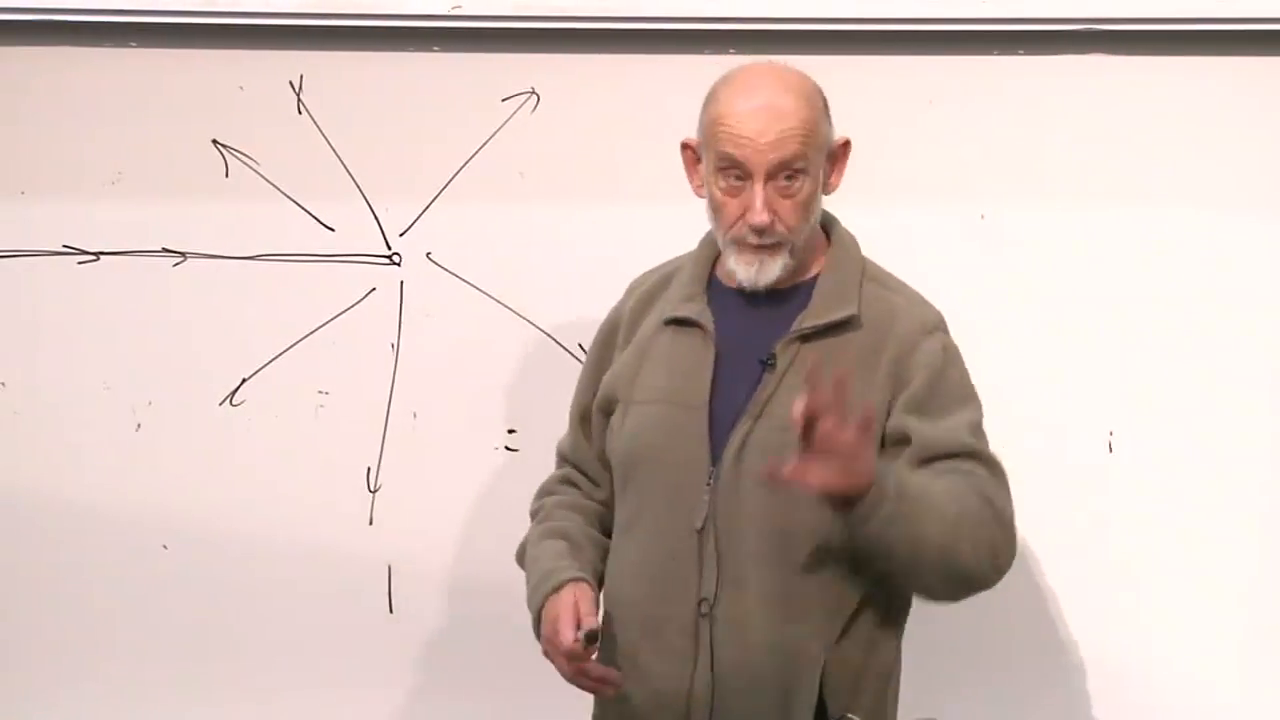
\includegraphics[width=0.84\textwidth]{lecture_10_figure_10.png}
\caption{黒板に描かれた細いソレノイドの描像：磁力線は見かけの磁極から広がり、戻ってくる磁束は狭い管に閉じ込められている。}
\lectureframe{01:27:35}
\end{figure}

通常の古典電磁気学の範囲では、固定された磁束を消滅する断面積に押し込むと、場の強さと場のエネルギーが増大する。講義では、現実的な単磁極には通常のソレノイドをどんどん細くするだけではなく新しい物理が必要であることを強調するために、無限のエネルギーについての意図的に誇張した応答を用いている。量子論では、適切に量子化された磁束管はその芯の外側では観測不能になりうる。これがディラック弦の構成の背後にある考え方であるが、完全な単磁極の理論は本講義の範囲を超えている。

\begin{classroomqa}
\audiencequestion{点粒子は磁気モーメントをもちうる。それは単磁極か。}
\lecturerresponse{いいえ。磁気モーメントは双極子である。すなわち、等しく反対の極性をもつ。単磁極は一つの正味の磁荷を担うであろう。通常の磁石を切ってもその極は分離されず、各部分がそれぞれ自分のN極とS極を獲得する。}
\end{classroomqa}

\begin{classroomqa}
\audiencequestion{二つの端を分離することの困難さは、クォークの閉じ込めに類似しているか。}
\lecturerresponse{それは有用な類推である。閉じ込められたクォークを引き離しても、通常の観測では孤立したクォークは得られず、つなぐ場が新たな束縛された対象を生み出す。ここで両者の機構を同一視しているわけではないが、避けがたい磁束構造で結ばれた端点という描像は似ている。}
\end{classroomqa}

講義の結論は慎重である。磁気単極子は、この導出で用いた通常の古典理論の一部ではないが、多くの高エネルギー理論はそれを含んでいる。もしそれらが素粒子として存在するならば、この教室の力学をはるかに超えるエネルギー・スケールが関与すると予想される。

\section{ハミルトンのもう一つの代数と未完成の話題}

最後に聴衆からの質問が、ハミルトンの四元数について尋ねる。それらは歴史的にはハミルトン力学とは別個のものである。ハミルトンは、複素数が平面内の回転に対して果たす役割に似た何かを三次元回転に対して果たしうる代数を求めた。その結果は三つの虚数単位 \(i,j,k\) を用い、
\begin{equation}
  i^2=j^2=k^2=ijk=-1,
\end{equation}
であり、たとえば
\begin{equation}
  ij=k,
  \qquad
  ji=-k.
\end{equation}
である。単位四元数は三次元回転の効率的な表現を与える。量子力学では、同じ代数構造を、通常の虚数単位の適切な因子とともにパウリ行列で表すことができる。この関連は実在するが、本講義で展開した正準運動量やハミルトニアンの起源ではない。

最後に要望された話題はカオスである。それを展開する時間は残っていない。講義は、すでに構築した道具立てを振り返って閉じられる。すなわち、力学とは位相空間における軌道に沿った運動であり、その言葉が規則的およびカオス的振る舞いを研究するための出発点である。古典力学の形式的構造は、聴衆がそこから先へ進むのに十分なほど完成している。
